\chapter{Evaluation}
\label{cha:evaluation}

% In this chapter we will evaluate the implementation of environments in the PROCEED MS,
% for this we will go through the requirements defined in \ref{cha:tasklist}.
% The primary goals of this thesis were to introduce environments as isolated workspaces for personal and organizational use,
% enable efficient asset management through a hierarchical folder structure,
% and adapt the MS's a role-based access control system to fit environments.
% The following \ref{fig:task-list-functional-quick-evaluation} table shows a quick rundown of the evaluation.
In this chapter, we evaluate the implementation of environments in the PROCEED MS by
reviewing the requirements defined in section \ref{cha:tasklist}.
The primary goals were to introduce isolated workspaces for both personal and organizational use,
enable efficient asset management through a hierarchical folder structure, and adapt the role-based access
control system to support these new workspaces.
Table \ref{fig:task-list-functional-quick-evaluation} provides an overview of the task statuses:

\begin{figure}[H]
	\centering

	\begin{tabular}{ | m{20em} | m{17em}| }
		\hline
		 Task & Status \\
     \hline
      1. Implement environments &  Partially implemented: folders were only implemented for processes. \\
     \hline
      2. Personal and organization Environments &  Implemented \\
     \hline
      3. Adapt the MS' user management system to fit environments &  Implemented \\
     \hline
      4. Adapt the MS' role system to fit environments &  Implemented \\
     \hline
  %    1.a & x \\
		%  1.b &  \\
		%  1.c &  \\
		%  1.d &  \\
		%
		%  2.a &  \\
		%  2.b &  \\
		%  2.c &  \\
		%  2.d &  \\
		%  2.e &  \\
		%  2.f &  \\
		%  2.g &  \\
		%  3.a & \\
		%
		%  3.b.i &  \\
		%
		%  3.b.ii &  \\
		%  3.b.iii &  \\
		%  3.b.iv &  \\
		%  3.c &  \\
		%  3.d &  \\
		%
		%  4.a &  \\
		%  4.b &  \\
		%  4.c &  \\
		%  4.d &  \\
		%  4.e &  \\
		% ------------------------------------------------------------------------------
	\end{tabular}

	\caption{Evaluation of Task List.}
	\label{fig:task-list-functional-quick-evaluation}
\end{figure}

According to \textbf{task 1} Environments are stored as entries in the MS's storage
solution with a unique id.
Every asset in the MS explicitly stores the id of the environment it belongs to.
Memberships to environments are stored in a separate table, where each entry has a user id
and an environment id,
later on we will explain how the access to assets is managed.
Furthermore, each environment has a root folder, which contains more folders and
processes.
Apart from root folders, both process and folders store the id of the folder they belong
to.

According to \textbf{task 2} environments store a flag to determine whether they are a
personal or an organization environment.
Personal environments are created when a user is created and organization environments can
be created by signed-in users.
Personal environments have a restricted feature-set, this is enforced by the role
system, this will be explained in more detail when we address task 4.
Users in organization environments can potentially use all the MS's features, this is
determined by the roles they have inside that environment.
The user that creates an organization environment is assigned the role of admin inside
that environment.
Access to assets in organization environments is managed by the role system described in
task 4,
the admin role has all permissions for all assets in the environment.
Organization environments can have multiple members, new members can be invited by other
members with the right permissions.

According to \textbf{task 3}, the user management was redesigned to accommodate
multi-tenancy,
users are now stored as records in the MS's storage solution independently of the environments they belong to.
This allows for them to be part of multiple environments.
Users also have the option to sign in as a guest, which allows them to try the MS inside
a personal environment without having to sign up.
Guest users are stored as other users, but with a flag that indicates that they are a
guest.

According to \textbf{task 4}, the MS's role system was adapted to fit environments and
folders. In its essence, roles work as they do before with two key differences:
Each role belongs to an environment and is only applied for assets inside that
environment, and roles can be scoped to folders, meaning that its permissions apply on all
descendants of the folder.
The role system was also leveraged to restrict the feature set of personal environments:
while personal environments don't have roles, the MS still uses the role system to manage
access to assets inside personal environments, it gives the owner of the environment all
permissions for the allowed features and restricts the rest.

\ref{cha:tasklist} also describes a set of non-functional requirements mostly related to
developer experience.
In contrast to functional requirements, which can be evaluated by determining weather the
task was completed or not,
non-functional requirements are harder to evaluate, as they are subjective.
For this reason we determined that surveying the developers that are working on the MS
would be the best way to evaluate these non-functional requirements.
The survey contained six questions, each question was meant to evaluate one of the
non-functional requirements.
Most questions were answered with a scale from 1 to 5, for some questions 1 meant that the
task was perfectly achieved and for others it was the opposite.
For these questions the task is considered as sufficiently met if the average of the
answers tends to the favorable side.

%Script for downloading svgs
%async function downloadSVGAsPNG(svgElement, fileName = 'image.png') {
%  const svgData = new XMLSerializer().serializeToString(svgElement);
%  const svgBlob = new Blob([svgData], { type: 'image/svg+xml;charset=utf-8' });
%
%  const url = URL.createObjectURL(svgBlob);
%  const img = new Image();
%
%  img.onload = () => {
%    const canvas = document.createElement('canvas');
%    canvas.width = svgElement.clientWidth;
%    canvas.height = svgElement.clientHeight;
%
%    const context = canvas.getContext('2d');
%    context.drawImage(img, 0, 0);
%
%    canvas.toBlob((blob) => {
%      const pngUrl = URL.createObjectURL(blob);
%      const downloadLink = document.createElement('a');
%      downloadLink.href = pngUrl;
%      downloadLink.download = fileName;
%      document.body.appendChild(downloadLink);
%      downloadLink.click();
%      document.body.removeChild(downloadLink);
%      URL.revokeObjectURL(pngUrl);
%    }, 'image/png');
%
%    URL.revokeObjectURL(url);
%  };
%
%  img.src = url;
%}

% --------------------------------------------------
% Non-functional 1: changes to the MS
% --------------------------------------------------

Non-functional requirement 1 was to keep the changes to the MS to a minimum, to evaluate
this the survey asked:
"On a scale of 1 (very minimal) to 5 (extensive), how significantly do you feel the
codebase had to change to support multi-tenant environments?".
Figure \ref{fig:evaluation:non-functional:1} shows a histogram of the answers to this question.
The answers lie mostly in the middle, with a slight tendency towards the lower end of the
scale, thus we conclude that this task was sufficiently met.

\begin{figure}[h]
	\centering
  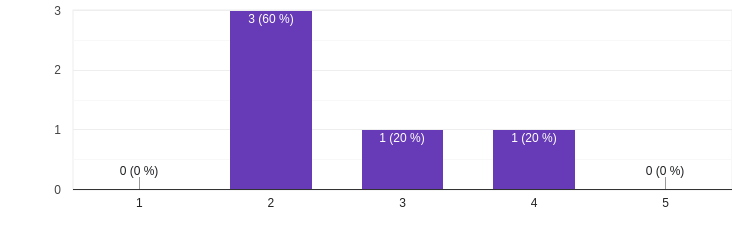
\includegraphics[scale=0.55]{../../figures/survey/1-changes-ms.png}
	\caption{Histogram of answers to the question: "On a scale of 1 (very minimal) to 5
  (extensive), how significantly do you feel the codebase had to change to support
  multi-tenant environments?"}
	\label{fig:evaluation:non-functional:1}
\end{figure}

% --------------------------------------------------
% Non-functional 2: intuitive ui
% --------------------------------------------------

Non-functional requirement 2 was to provide an intuitive user interface, 
to evaluate this the survey asked: 
"On a scale of 1 (not intuitive at all) to 5 (extremely intuitive), how would you
rate the ease of navigating and managing folders/environments in the new UI?".
Figure \ref{fig:evaluation:non-functional:2} shows a histogram of the answers to this question.
The answers lie mostly in the upper end of the scale, thus we conclude that the user
interface is sufficiently intuitive.

\begin{figure}[h]
	\centering
  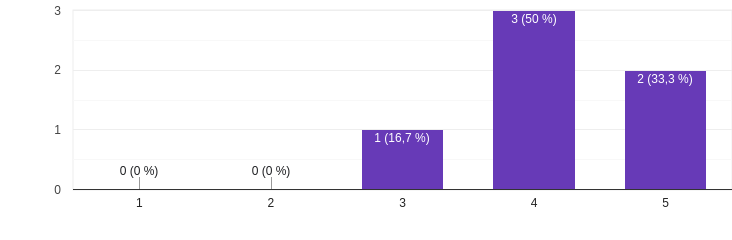
\includegraphics[scale=0.55]{../../figures/survey/2-ui.png}
	\caption{Histogram of answers to the question: "On a scale of 1 (not intuitive at all) to 5 (extremely intuitive), how would you
rate the ease of navigating and managing folders/environments in the new UI?"}
	\label{fig:evaluation:non-functional:2}
\end{figure}

% --------------------------------------------------
% Non-functional 3.a: share code
% --------------------------------------------------

Non-functional requirement 3.a was that personal and organization environments share the
same data structures and functions, to improve the developer experience.
To evaluate this the survey asked a yes or no question:
"Do you feel that personal and organization environments share sufficiently unified
structures and functions to use them?".
The six developers that answered this question answered "yes", thus we conclude that this
task requirement was met.

% --------------------------------------------------
% Non-functional 3.b: intuitive ui
% --------------------------------------------------

Non-functional requirement 3.b was to choose a simple data structure for the folder
system and to provide simple functions to manage it.,
To evaluate this the survey asked: 
"On a scale of 1 (very simple) to 5 (overly complex), how would you rate the
complexity of the folder system’s data model and its related functions?"
Figure \ref{fig:evaluation:non-functional:3.2} shows a histogram of the answers to this question.
Four people answered "2" and two people answered "3", thus we conclude the user interface
is sufficiently intuitive.


\begin{figure}[h]
	\centering
  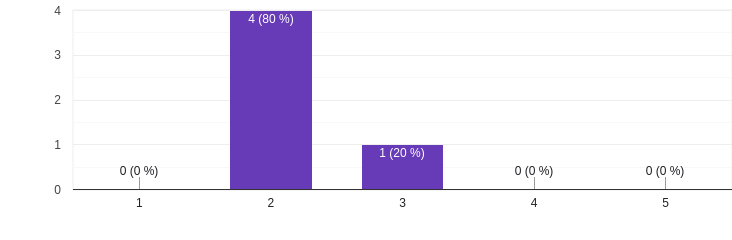
\includegraphics[scale=0.55]{../../figures/survey/3.2-folder-structures.png}
	\caption{Histogram of answers to the question: "On a scale of 1 (very simple) to 5 (overly complex), how would you rate the
complexity of the folder system’s data model and its related functions?"}
	\label{fig:evaluation:non-functional:3.2}
\end{figure}

% --------------------------------------------------
% Non-functional 3.c: backend functions for permissions
% --------------------------------------------------

Non-functional task 3.c was to streamline environment identification and permissions check in the backend.
To evaluate this the survey asked: 
"On a scale of 1 (not at all effective) to 5 (extremely effective), how effective are the
new backend helper functions in streamlining environment identification and permission
checks?"
Figure \ref{fig:evaluation:non-functional:3.3} shows a histogram of the answers to this question.
One person voted "3" and the rest of votes where in the favorable side of the scale,
thus we conclude that this task was sufficiently met.

\begin{figure}[h]
	\centering
  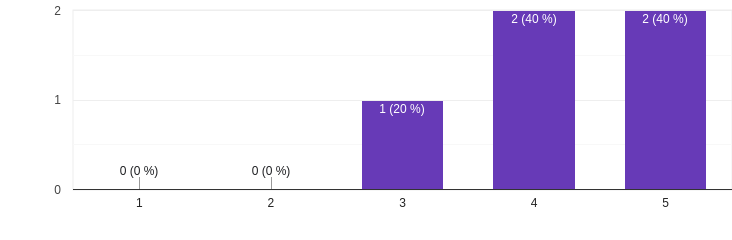
\includegraphics[scale=0.55]{../../figures/survey/3.3-backend-permissions.png}
	\caption{Histogram of answers to the question: "On a scale of 1 (not at all effective) to 5 (extremely effective), how effective are the
new backend helper functions in streamlining environment identification and permission checks?"}
	\label{fig:evaluation:non-functional:3.3}
\end{figure}

% --------------------------------------------------
% Non-functional 3.d: backend functions for permissions
% --------------------------------------------------

Non-functional task 3.d was to introduce simpler helper functions for the frontend, to adapt
the interface to a user's permissions within an environment. To evaluate this the survey asked: 
"On a scale of 1 (no change in complexity) to 5 (drastically simpler), how much do the new
frontend helper functions simplify adapting UI elements based on each user’s
permissions?"
Figure \ref{fig:evaluation:non-functional:3.4} shows a histogram of the answers to this question.
One person voted "3" and the rest of votes where in the favorable side of the scale,
thus we conclude that this task was sufficiently met.

\begin{figure}[h]
	\centering
  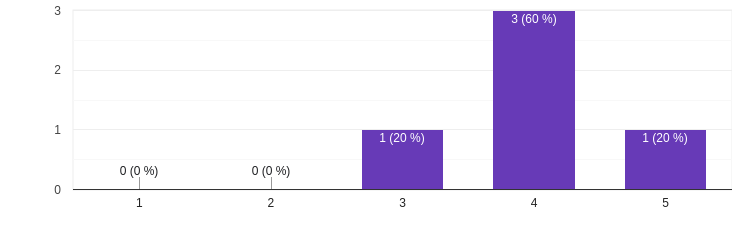
\includegraphics[scale=0.55]{../../figures/survey/3.4-frontend-permissions.png}
	\caption{Histogram of answers to the question: "On a scale of 1 (no change in complexity) to 5 (drastically simpler), how much do the new
frontend helper functions simplify adapting UI elements based on each user’s
permissions?"}
	\label{fig:evaluation:non-functional:3.4}
\end{figure}


% \begin{figure}[H]
% 	\centering
%
% 	\begin{tabular}{ | m{10em} | m{25em}| m{4em} |}
% 		\hline
%      Task & Question & Answer \\
%      \hline
%       1. Keep changes to a minimum. &
%       On a scale of 1 (very minimal) to 5 (extensive), how significantly do you feel the
%       codebase had to change to support multi-tenant environments? &
%       4\\
%      \hline
%       2. Intuitive user interface &  
%       On a scale of 1 (not intuitive at all) to 5 (extremely intuitive), how would you
%       rate the ease of navigating and managing folders/environments in the new UI? &
%       5\\
%      \hline
%       3. Choose simple data structures. & & \\
%      \hline
%       3.1 Share data structures between personal and organization environments &  
%       Do you feel that personal and organization environments share sufficiently unified
%       structures and functions to use them? &
%       5 \\
%      \hline
%       3.2 Simple data structures for folders &  
%       On a scale of 1 (very simple) to 5 (overly complex), how would you rate the
%       complexity of the folder system’s data model and its related functions? &
%       5\\
%      \hline
%       3.3 Simple backend functions to enforce role permissions &   
%       On a scale of 1 (not at all effective) to 5 (extremely effective), how effective are the
%       new backend helper functions in streamlining environment identification and permission
%       checks? &
%       4 \\
%       \hline
%       3.4 Simple frontend functions to adapt UI to a user's permissions &  
%       On a scale of 1 (no change in complexity) to 5 (drastically simpler), how much do the new
%       frontend helper functions simplify adapting UI elements based on each user’s
%       permissions? &
%       \\
%      \hline
% 	\end{tabular}
	% \caption{Evaluation of Task List.}
	% \label{fig:task-list-non-functional-quick-evaluation}
% \end{figure}
